
\section{Experiments}
\label{sec:experiments}

\par In this section, we explore the challenges of action and return conditioned imitation learning and provide results for the Can and Lift tasks. We investigate the effects of introducing inaccuracies at test-time by conditioning the policy on its own slightly inaccurate history of actions and return-to-go values. Our experiments show that these inaccuracies can lead to lower task success rates for Decision Transformers (DT) compared to behavior cloning (BC) baselines. We then train DT models with various context sequence lengths on the more difficult "All" data setting of the Can task and show that longer context sequences improve prediction accuracy. Finally, we compare DT against BC baselines on the mixed-quality ``All" dataset, demonstrating the effectiveness of DT's return-conditioning and context sequences for imitation learning in complex environments.

\subsection{Understanding the Challenges of Action and Return-Conditioned Imitation Learning}
\label{sec:challenges}
Decision Transformers condition their outputs on a fixed-length history of previous actions, return-to-go scalars, and observations. While this may help differentiate between the various demonstrators in a mixed-quality dataset, it also introduces new opportunities for distributional shifts during evaluation: at test-time, the policy is conditioned on the history of its own (slightly inaccurate) actions and return-to-go values. These inaccuracies can compound over the length of a trajectory, potentially causing DT to achieve a lower task success rate than a BC baseline. As a first step, we investigate this effect on the Can placement task using only the highest quality dataset of human demonstrations (PH). In this setting, DT's ability to learn from mixed-quality data is less relevant. We use context lengths of one to compare directly against BC, meaning that the input to a DT model during evaluation is the most recent state, action, and return-to-go. We can optionally hide the action and/or RTG information. Hiding actions and RTGs recover the simple BC baseline, and a context length of one makes the attention component of the Transformer redundant. 

Success rates are measured by pausing training and evaluating the current policy in the robomimic environment simulator. The success rates of several ablations of DT input format over the course of training are plotted in Figure \ref{fig:can_ph_success_rates}. While standard BC matches the performance of the demonstrations and the original robomimic baselines, DT variants that introduce action and RTG inputs can struggle to achieve expert results. Increasing model size appears to improve performance by outputting more accurate actions and being more robust to variations in the input.

\begin{figure}
    \centering
    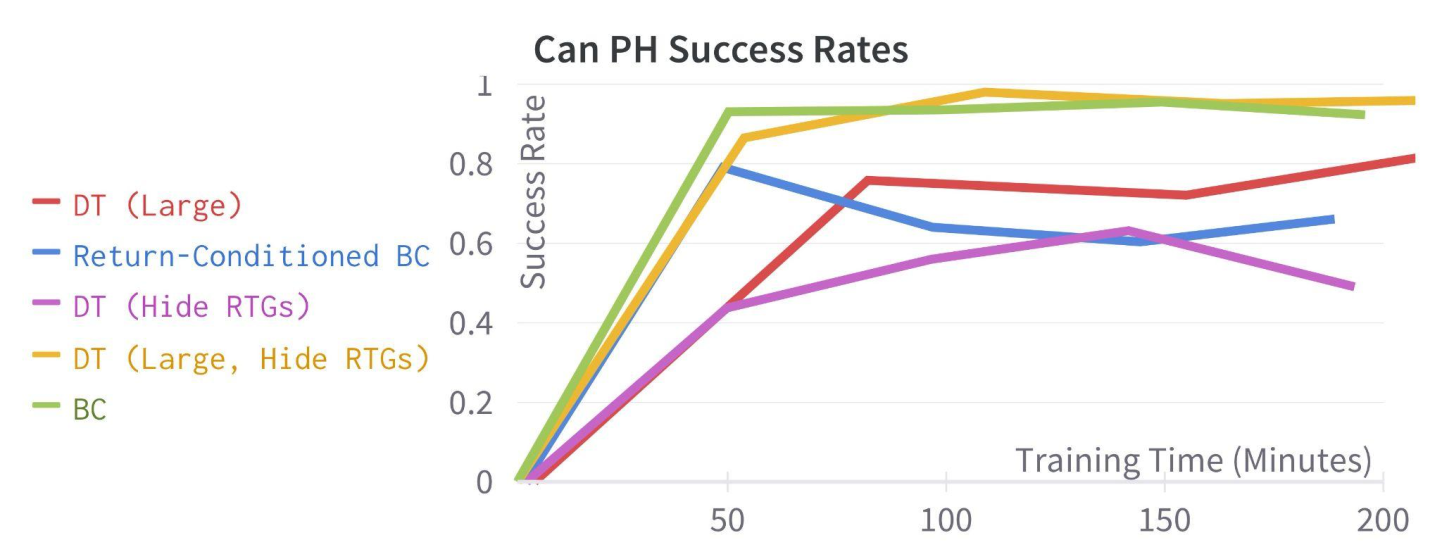
\includegraphics[width=\linewidth]{figs/can_ph_success_rates.png}
    \caption{Success rate of ablations of the DT input format in the Can task using only the highest quality PH data. ``Large" policies double the networks' embedding and feedforward dimensions.}
    \label{fig:can_ph_success_rates}
\end{figure}

\subsection{Decision Transformer on Can and Lift Tasks}
Although action and RTG inputs may harm performance at test-time, our next experiment investigates whether DT's sequence inputs improve the accuracy of action predictions during training. We train identical DT agents with context lengths of $3, 10$ and $20$ on the more difficult ``All" data setting of the Can task. We would expect longer context sequence lengths to improve prediction accuracy by providing more information on the quality and action choices of the demonstrator that created each training sequence. The negative log-likelihood training loss (Equation \ref{eq:loss}) for the three models is plotted in Figure \ref{fig:can_all_train_loss}. Despite equal model sizes, regularization, and optimization settings, DT's fit of the training data improves with context sequence length. 

\begin{figure}
    \centering
    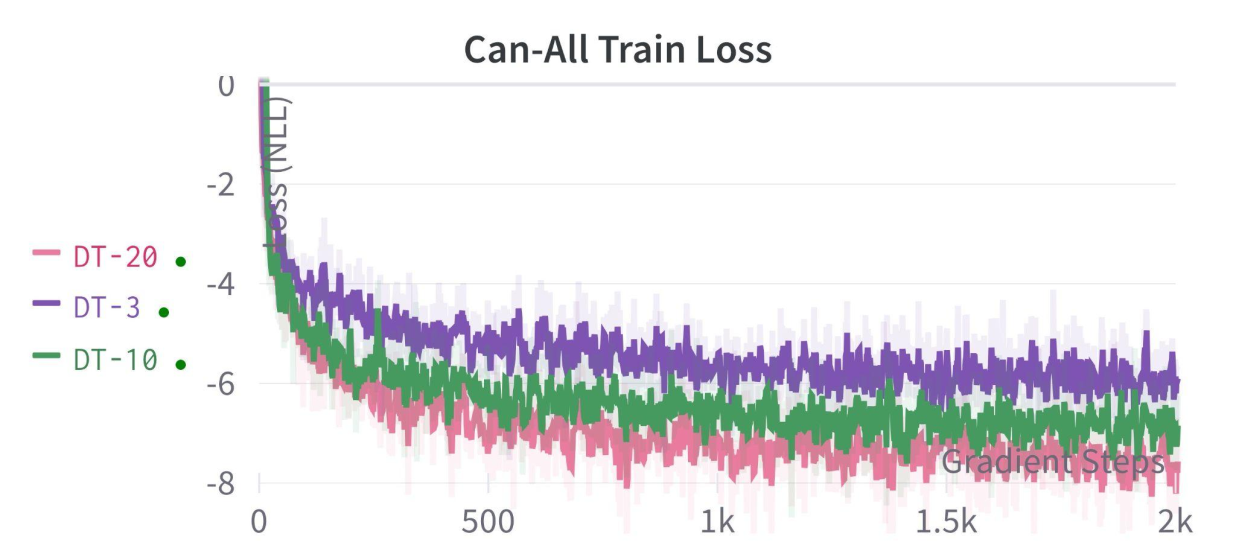
\includegraphics[width=\linewidth]{figs/can_all_train_loss.png}
    \caption{Training Loss of DT with context lengths of $3, 10$ and $20$. Longer context sequences improve action predictions by resolving ambiguity about which demonstrator is being imitated.}
    \label{fig:can_all_train_loss}
\end{figure}

Next, we conduct a larger-scale evaluation of DT with various context lengths and policy types. We compare against simpler BC baselines on the mixed-quality ``All" dataset types consisting of both low-quality machine-generated data and high-quality human demonstrations. The results for the Lift task are shown in Table \ref{tbl:liftresults}, where DT-$k$ denotes our Decision Transformer model with a context sequence of length $k$. Because DT is conditioned on the return-to-go values of its training data, we need to select a target return to imitate at test-time. We settle on the simple heuristic of finding the $95$th percentile of the returns in the training dataset. We explore this choice further in Section \ref{sec:expreturnsweep}. The \textit{Naive BC} method uses a Gaussian policy without context sequences or return-conditioning and achieves a success rate of just $35\%$ - highlighting the challenges of imitation learning from mixed-quality datasets with multiple demonstrators. For comparison, the original robomimic BC results achieve a success rate of $100\%$ using the PH data and $65\%$ from the lowest-quality MG data. We replicate these experiments with our codebase and report success rates of $99\%$ for \textit{Naive BC} on PH data. This suggests that learning from the mixed ``All" dataset is more difficult than learning from any of its sub-components as a result of multi-modality. DT uses return-conditioning to filter dataset quality and context sequences to resolve multi-modality. As a sanity check, we train DT-$1$ on the PH data with $100\%$ success. DT-$1$ still sees a decrease in performance on the ``All" dataset but uses its return-conditioning to improve significantly on the BC baseline with a success rate of $85\%$. By extending the context sequence to $20$ timesteps, DT-$20$ can further improve to $94\%$.

\begin{table*}[]
\centering
\caption{\textbf{Lift-All Results}}
\resizebox{.8\textwidth}{!}{
\begin{tabular}{@{}lccccccc@{}}
\toprule
 & Naive BC & \begin{tabular}[c]{@{}c@{}}BC +\\ Action Inp.\end{tabular} & \begin{tabular}[c]{@{}c@{}}DT-1 \\ (PH Only)\end{tabular} & DT-1 & DT-3 & DT-10 & DT-20 \\ \midrule
Success Rate (\%) & 35 & 20 & \textit{100} & 85 & 92 & 92 & \textbf{94} \\
Return & 189 & 113 & \textit{463} & 397 & 428 & \textbf{433} & 421 \\ \bottomrule
\end{tabular}
}
\label{tbl:liftresults}
\end{table*}

Table \ref{tbl:canresults} shows the results of a similar experiment on the Can task. Although we successfully replicate the near-perfect success rate of the original robomimic results on the PH data, Naive BC once again fails ($14\%$) on our mixed dataset. The relative performance of the methods on Can is similar to Lift, although we find the return and action conditioning to have a negative impact on this task as noted in Section \ref{sec:challenges}. \hspace{7mm} DT-$3$ achieves the highest performance on Can-All with a task success rate of $81\%$. Further discussion of the challenges in recovering the $100\%$ success rate of the PH dataset with our Decision Transformer model is provided in Section \ref{sec:discussion}.



\begin{table*}[]
\centering
\caption{\textbf{Can-All Results}}
\resizebox{.8\textwidth}{!}{
\begin{tabular}{@{}lcccccc@{}}
\toprule
 & \begin{tabular}[c]{@{}c@{}}BC \\ (PH Only)\end{tabular} & Naive BC & \begin{tabular}[c]{@{}c@{}}BC + \\ Action Inp.\end{tabular} & DT-3 & DT-10 & DT-20 \\ \midrule
Success Rate (\%) & \textit{99} & 14 & 15 & \textbf{81} & 76 & 63 \\
Return & \textit{396} & 72 & 74 & \textbf{362} & 337 & 286 \\ \bottomrule
\end{tabular}
}
\label{tbl:canresults}
\end{table*}


\subsection{Ablations}
There are two key implementation details that affect the performance of the Decision Transformer which could benefit from further analysis. First is the size of the Transformer architecture. While massive multi-billion parameter Transformers have been essential for progress in language modeling \cite{brown2020language} when learning from internet-scale datasets, recent applications of Transformers to RL and robotic control problems have preferred much smaller model sizes \cite{shafiullah2022behavior, decisiontransformer, cui2022play}. We compare the performance of the larger Transformer used in the main Can-All experiments (Table \ref{tbl:canresults}) - which used an embedding dimension of $512$, a feedforward dimension of $2048$, and $4$ Transformer layers - with a smaller architecture of $3$ layers with embedding dimension $200$ and feedforward dimension $800$. The smaller architecture is the same as was used for the easier Lift-All experiments (Table \ref{tbl:liftresults}). The results are shown in Table \ref{tbl:modelsizes}. The larger model appears to provide a meaningful improvement in performance across all three context lengths. Because expert human demonstrations are expensive to collect, related work in Transformers for robotic imitation learning uses architectures much smaller than even our ``Small" model to prevent overfitting. DT's return-conditioning offers a promising way to make use of diverse experiences and benefit from the generalization of large networks.

\begin{table}[h!]
\caption{\textbf{DT Network Sizes on Can-All}}
\resizebox{\columnwidth}{!}{
\begin{tabular}{@{}lccccccc@{}}
\toprule
 & \begin{tabular}[c]{@{}c@{}}DT-3 \\ (Large)\end{tabular} & \begin{tabular}[c]{@{}c@{}}DT-10 \\ (Large)\end{tabular} & \begin{tabular}[c]{@{}c@{}}DT-20 \\ (Large)\end{tabular} & \begin{tabular}[c]{@{}c@{}}DT-3 \\ (Small)\end{tabular} & \begin{tabular}[c]{@{}c@{}}DT-10\\  (Small)\end{tabular} & \begin{tabular}[c]{@{}c@{}}DT-20 \\ (Small)\end{tabular} & \begin{tabular}[c]{@{}c@{}}DT-3 \\ (Large, Gaussian)\end{tabular} \\ \midrule
Success Rate (\%) & \textbf{81} & 76 & 63 & 65 & 57 & 61 & 66 \\
Return & \textbf{362} & 337 & 286 & 292 & 262 & 278 & 204 \\ \bottomrule
\end{tabular}
}
\label{tbl:modelsizes}
\end{table}

\begin{table}[h!]
\caption{\textbf{GMM vs. Gaussian on Lift-All}}
\resizebox{\columnwidth}{!}{
\begin{tabular}{@{}lcccccc@{}}
\toprule
              & DT-3 & DT-10 & DT-20 & \begin{tabular}[c]{@{}c@{}}DT-3\\  (Gaussian)\end{tabular} & \begin{tabular}[c]{@{}c@{}}DT-10 \\ (Gaussian)\end{tabular} & \begin{tabular}[c]{@{}c@{}}DT-20 \\ (Gaussian)\end{tabular} \\ \midrule
Success Rate (\%) & 92   & 92    & \textbf{94}    & 85                                                         & 86                                                          & 81                                                          \\
Return            & 428  & \textbf{433}   & 421   & 403                                                        & 406                                                         & 386                                                         \\ \bottomrule
\end{tabular}
}
\label{tbl:gmmgaussian}
\end{table}

Next, we compare two choices of policy parameterization. The independent Gaussian policy is widely used in the RL literature for continuous control. However, the multi-modal policies created by a mixture of human demonstrations may benefit from a more expressive policy. We include a Gaussian Mixture Model (GMM) policy and enable it by default in all previous experiments with the exception of Naive BC. In Table \ref{tbl:gmmgaussian}, we directly compare the two policy choices at three context lengths on the Lift-All task, where GMM outperforms the Gaussian alternative in all cases. In general, we would expect the gap between the two policy choices to decrease as the context length grows and the action sequence becomes more specific to a single demonstrator and therefore less multi-modal. 



\subsection{Return-Conditioning}
Because Decision Transformer models the actions of a range of policies of different quality, we are forced to select a ``target return" or initial RTG that creates the first input token of the context sequence. While the target return can be difficult to select in an online setting \cite{online_decisiontransformer, udrl_implementation}, in our offline case we can make an informed decision by looking at the distribution of returns available to us in the dataset. All results so far have used the heuristic of replicating the $95$th percentile of the returns in the training data. This decision was motivated by our desire to replicate high-quality behavior while staying safely inside the distribution of the training data. However, we can experiment with other choices of initial RTG. We evaluate trained policies across a range of target returns and plot the results in Figure \ref{fig:success_rate_curve}. Because standard BC is not return-conditioned, the target return has no effect and the policy performs equally poorly in all conditions. Adding the target return as an extra input to BC does allow for adaptation to multiple levels of quality; as our target return increases so does the actual return (Fig. \ref{fig:success_rate_curve} left) and success rate (Fig. \ref{fig:success_rate_curve} right). Decision Transformer uses its context sequence to improve action predictions and more closely matches the target return than return-conditioned BC. Note that all policies significantly underperform the target return at the lowest quality levels ($360-400$). We speculate that this discrepancy is caused by difficulty in accurately mimicking low-return policies as a result of the way our custom reward function is correlated with demonstration length. It may be challenging to replicate slow solutions to the task with a limited context sequence and without time information in the state representation. 

\label{sec:expreturnsweep}
\begin{figure}
    \centering
    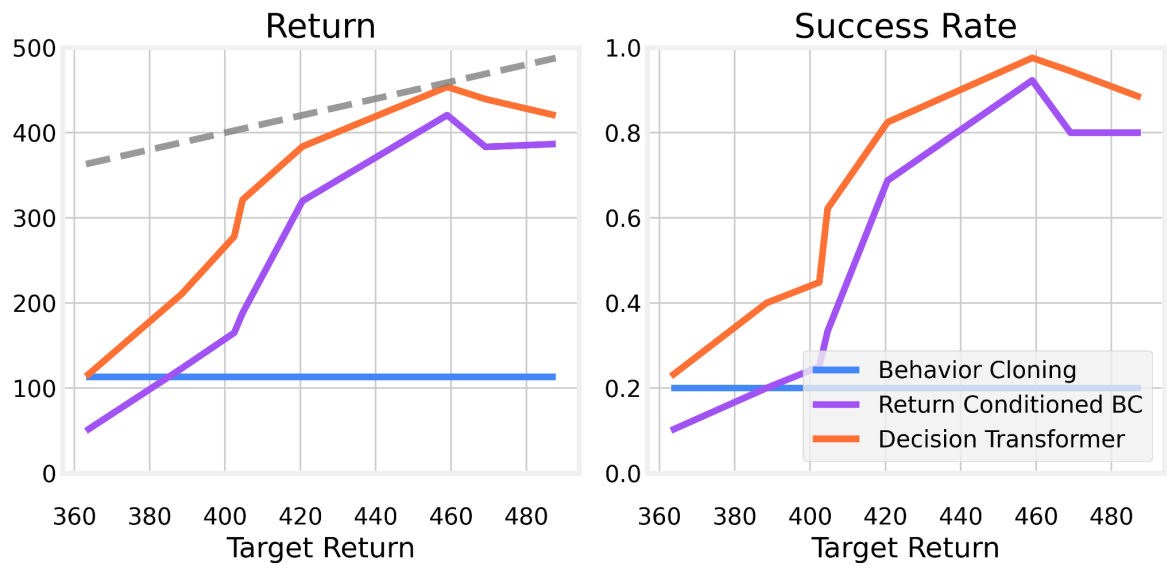
\includegraphics[width=\columnwidth]{figs/success_rate_curve.png}
    \caption{Return-conditioned policies replicate a range of performance qualities. As the target return increases, so does the actual return and success rate of the agents.} 
    \label{fig:success_rate_curve}
\end{figure}